\begin{figure}[H] \centering % Created by tikzDevice version 0.12.4 on 2023-07-16 16:34:05
% !TEX encoding = UTF-8 Unicode
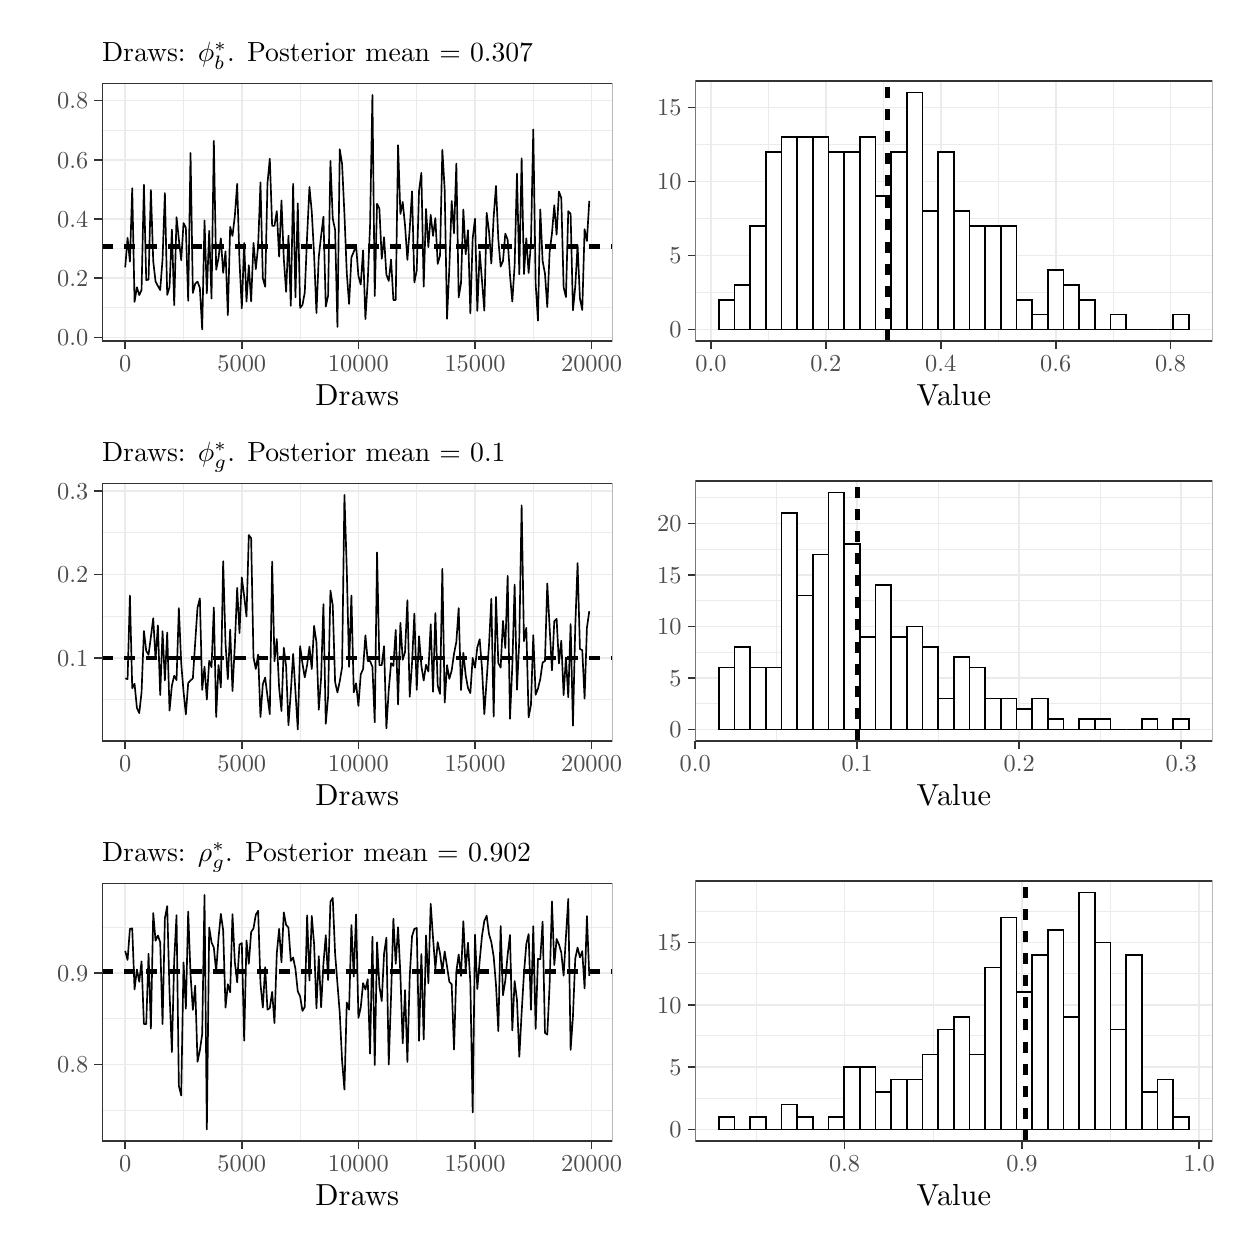
\begin{tikzpicture}[x=1pt,y=1pt]
\definecolor{fillColor}{RGB}{255,255,255}
\path[use as bounding box,fill=fillColor,fill opacity=0.00] (0,0) rectangle (433.62,433.62);
\begin{scope}
\path[clip] (  0.00,289.08) rectangle (216.81,433.62);
\definecolor{drawColor}{RGB}{255,255,255}
\definecolor{fillColor}{RGB}{255,255,255}

\path[draw=drawColor,line width= 0.6pt,line join=round,line cap=round,fill=fillColor] (  0.00,289.08) rectangle (216.81,433.62);
\end{scope}
\begin{scope}
\path[clip] ( 26.87,320.33) rectangle (211.31,413.52);
\definecolor{fillColor}{RGB}{255,255,255}

\path[fill=fillColor] ( 26.87,320.33) rectangle (211.31,413.52);
\definecolor{drawColor}{gray}{0.92}

\path[draw=drawColor,line width= 0.3pt,line join=round] ( 26.87,332.36) --
	(211.31,332.36);

\path[draw=drawColor,line width= 0.3pt,line join=round] ( 26.87,353.78) --
	(211.31,353.78);

\path[draw=drawColor,line width= 0.3pt,line join=round] ( 26.87,375.20) --
	(211.31,375.20);

\path[draw=drawColor,line width= 0.3pt,line join=round] ( 26.87,396.62) --
	(211.31,396.62);

\path[draw=drawColor,line width= 0.3pt,line join=round] ( 56.32,320.33) --
	( 56.32,413.52);

\path[draw=drawColor,line width= 0.3pt,line join=round] ( 98.45,320.33) --
	( 98.45,413.52);

\path[draw=drawColor,line width= 0.3pt,line join=round] (140.58,320.33) --
	(140.58,413.52);

\path[draw=drawColor,line width= 0.3pt,line join=round] (182.70,320.33) --
	(182.70,413.52);

\path[draw=drawColor,line width= 0.6pt,line join=round] ( 26.87,321.65) --
	(211.31,321.65);

\path[draw=drawColor,line width= 0.6pt,line join=round] ( 26.87,343.07) --
	(211.31,343.07);

\path[draw=drawColor,line width= 0.6pt,line join=round] ( 26.87,364.49) --
	(211.31,364.49);

\path[draw=drawColor,line width= 0.6pt,line join=round] ( 26.87,385.91) --
	(211.31,385.91);

\path[draw=drawColor,line width= 0.6pt,line join=round] ( 26.87,407.33) --
	(211.31,407.33);

\path[draw=drawColor,line width= 0.6pt,line join=round] ( 35.25,320.33) --
	( 35.25,413.52);

\path[draw=drawColor,line width= 0.6pt,line join=round] ( 77.38,320.33) --
	( 77.38,413.52);

\path[draw=drawColor,line width= 0.6pt,line join=round] (119.51,320.33) --
	(119.51,413.52);

\path[draw=drawColor,line width= 0.6pt,line join=round] (161.64,320.33) --
	(161.64,413.52);

\path[draw=drawColor,line width= 0.6pt,line join=round] (203.77,320.33) --
	(203.77,413.52);
\definecolor{drawColor}{RGB}{0,0,0}

\path[draw=drawColor,line width= 0.6pt,line join=round] ( 35.25,347.02) --
	( 36.10,357.67) --
	( 36.94,349.04) --
	( 37.78,375.58) --
	( 38.62,334.53) --
	( 39.47,339.80) --
	( 40.31,337.01) --
	( 41.15,338.78) --
	( 42.00,376.86) --
	( 42.84,342.41) --
	( 43.68,342.57) --
	( 44.52,374.97) --
	( 45.37,349.24) --
	( 46.21,341.89) --
	( 47.05,340.30) --
	( 47.89,338.82) --
	( 48.74,349.99) --
	( 49.58,373.85) --
	( 50.42,337.05) --
	( 51.26,339.90) --
	( 52.11,360.69) --
	( 52.95,333.35) --
	( 53.79,365.13) --
	( 54.63,357.15) --
	( 55.48,349.57) --
	( 56.32,363.00) --
	( 57.16,361.34) --
	( 58.00,334.93) --
	( 58.85,388.36) --
	( 59.69,337.75) --
	( 60.53,341.09) --
	( 61.37,341.87) --
	( 62.22,339.58) --
	( 63.06,324.57) --
	( 63.90,363.92) --
	( 64.74,337.63) --
	( 65.59,360.19) --
	( 66.43,335.74) --
	( 67.27,392.73) --
	( 68.11,346.16) --
	( 68.96,350.36) --
	( 69.80,357.50) --
	( 70.64,345.02) --
	( 71.49,352.79) --
	( 72.33,329.71) --
	( 73.17,361.64) --
	( 74.01,358.38) --
	( 74.86,365.64) --
	( 75.70,377.16) --
	( 76.54,349.25) --
	( 77.38,332.22) --
	( 78.23,355.81) --
	( 79.07,334.62) --
	( 79.91,347.77) --
	( 80.75,334.67) --
	( 81.60,355.85) --
	( 82.44,346.37) --
	( 83.28,354.74) --
	( 84.12,377.72) --
	( 84.97,343.13) --
	( 85.81,340.01) --
	( 86.65,377.39) --
	( 87.49,386.26) --
	( 88.34,361.99) --
	( 89.18,362.01) --
	( 90.02,367.32) --
	( 90.86,350.85) --
	( 91.71,371.18) --
	( 92.55,350.14) --
	( 93.39,338.14) --
	( 94.23,358.46) --
	( 95.08,333.14) --
	( 95.92,377.15) --
	( 96.76,336.21) --
	( 97.60,370.13) --
	( 98.45,332.35) --
	( 99.29,333.42) --
	(100.13,337.94) --
	(100.98,358.42) --
	(101.82,376.04) --
	(102.66,367.08) --
	(103.50,351.43) --
	(104.35,330.51) --
	(105.19,350.85) --
	(106.03,358.36) --
	(106.87,365.31) --
	(107.72,332.82) --
	(108.56,336.83) --
	(109.40,385.46) --
	(110.24,364.65) --
	(111.09,360.55) --
	(111.93,325.47) --
	(112.77,389.67) --
	(113.61,384.32) --
	(114.46,366.27) --
	(115.30,345.07) --
	(116.14,333.77) --
	(116.98,350.61) --
	(117.83,352.66) --
	(118.67,354.87) --
	(119.51,343.92) --
	(120.35,340.79) --
	(121.20,353.15) --
	(122.04,328.32) --
	(122.88,341.99) --
	(123.72,362.09) --
	(124.57,409.29) --
	(125.41,336.64) --
	(126.25,369.96) --
	(127.09,368.22) --
	(127.94,350.11) --
	(128.78,357.88) --
	(129.62,344.38) --
	(130.47,342.10) --
	(131.31,349.85) --
	(132.15,335.19) --
	(132.99,335.24) --
	(133.84,391.15) --
	(134.68,366.30) --
	(135.52,370.61) --
	(136.36,362.14) --
	(137.21,349.72) --
	(138.05,360.92) --
	(138.89,374.48) --
	(139.73,341.54) --
	(140.58,345.89) --
	(141.42,374.67) --
	(142.26,381.13) --
	(143.10,340.04) --
	(143.95,368.11) --
	(144.79,354.33) --
	(145.63,365.98) --
	(146.47,358.38) --
	(147.32,364.81) --
	(148.16,348.25) --
	(149.00,351.27) --
	(149.84,389.49) --
	(150.69,374.92) --
	(151.53,328.39) --
	(152.37,346.87) --
	(153.21,370.98) --
	(154.06,359.31) --
	(154.90,384.47) --
	(155.74,336.18) --
	(156.58,341.23) --
	(157.43,367.92) --
	(158.27,351.75) --
	(159.11,360.46) --
	(159.96,330.39) --
	(160.80,357.42) --
	(161.64,364.58) --
	(162.48,331.28) --
	(163.33,352.76) --
	(164.17,342.17) --
	(165.01,331.38) --
	(165.85,366.68) --
	(166.70,360.04) --
	(167.54,348.38) --
	(168.38,365.19) --
	(169.22,376.39) --
	(170.07,357.07) --
	(170.91,347.28) --
	(171.75,349.30) --
	(172.59,359.20) --
	(173.44,357.01) --
	(174.28,344.22) --
	(175.12,334.67) --
	(175.96,347.75) --
	(176.81,380.84) --
	(177.65,344.48) --
	(178.49,386.43) --
	(179.33,344.57) --
	(180.18,357.49) --
	(181.02,344.96) --
	(181.86,355.82) --
	(182.70,396.85) --
	(183.55,341.19) --
	(184.39,327.75) --
	(185.23,367.91) --
	(186.07,349.34) --
	(186.92,344.77) --
	(187.76,332.69) --
	(188.60,352.41) --
	(189.45,359.30) --
	(190.29,369.44) --
	(191.13,358.79) --
	(191.97,374.41) --
	(192.82,372.09) --
	(193.66,339.83) --
	(194.50,336.26) --
	(195.34,367.31) --
	(196.19,366.35) --
	(197.03,331.50) --
	(197.87,340.04) --
	(198.71,355.09) --
	(199.56,335.73) --
	(200.40,331.60) --
	(201.24,360.78) --
	(202.08,356.54) --
	(202.93,371.00);

\path[draw=drawColor,line width= 1.7pt,dash pattern=on 4pt off 4pt ,line join=round] ( 26.87,354.53) -- (211.31,354.53);
\definecolor{drawColor}{gray}{0.20}

\path[draw=drawColor,line width= 0.6pt,line join=round,line cap=round] ( 26.87,320.33) rectangle (211.31,413.52);
\end{scope}
\begin{scope}
\path[clip] (  0.00,  0.00) rectangle (433.62,433.62);
\definecolor{drawColor}{gray}{0.30}

\node[text=drawColor,anchor=base east,inner sep=0pt, outer sep=0pt, scale=  0.88] at ( 21.92,318.62) {0.0};

\node[text=drawColor,anchor=base east,inner sep=0pt, outer sep=0pt, scale=  0.88] at ( 21.92,340.04) {0.2};

\node[text=drawColor,anchor=base east,inner sep=0pt, outer sep=0pt, scale=  0.88] at ( 21.92,361.46) {0.4};

\node[text=drawColor,anchor=base east,inner sep=0pt, outer sep=0pt, scale=  0.88] at ( 21.92,382.88) {0.6};

\node[text=drawColor,anchor=base east,inner sep=0pt, outer sep=0pt, scale=  0.88] at ( 21.92,404.30) {0.8};
\end{scope}
\begin{scope}
\path[clip] (  0.00,  0.00) rectangle (433.62,433.62);
\definecolor{drawColor}{gray}{0.20}

\path[draw=drawColor,line width= 0.6pt,line join=round] ( 24.12,321.65) --
	( 26.87,321.65);

\path[draw=drawColor,line width= 0.6pt,line join=round] ( 24.12,343.07) --
	( 26.87,343.07);

\path[draw=drawColor,line width= 0.6pt,line join=round] ( 24.12,364.49) --
	( 26.87,364.49);

\path[draw=drawColor,line width= 0.6pt,line join=round] ( 24.12,385.91) --
	( 26.87,385.91);

\path[draw=drawColor,line width= 0.6pt,line join=round] ( 24.12,407.33) --
	( 26.87,407.33);
\end{scope}
\begin{scope}
\path[clip] (  0.00,  0.00) rectangle (433.62,433.62);
\definecolor{drawColor}{gray}{0.20}

\path[draw=drawColor,line width= 0.6pt,line join=round] ( 35.25,317.58) --
	( 35.25,320.33);

\path[draw=drawColor,line width= 0.6pt,line join=round] ( 77.38,317.58) --
	( 77.38,320.33);

\path[draw=drawColor,line width= 0.6pt,line join=round] (119.51,317.58) --
	(119.51,320.33);

\path[draw=drawColor,line width= 0.6pt,line join=round] (161.64,317.58) --
	(161.64,320.33);

\path[draw=drawColor,line width= 0.6pt,line join=round] (203.77,317.58) --
	(203.77,320.33);
\end{scope}
\begin{scope}
\path[clip] (  0.00,  0.00) rectangle (433.62,433.62);
\definecolor{drawColor}{gray}{0.30}

\node[text=drawColor,anchor=base,inner sep=0pt, outer sep=0pt, scale=  0.88] at ( 35.25,309.32) {0};

\node[text=drawColor,anchor=base,inner sep=0pt, outer sep=0pt, scale=  0.88] at ( 77.38,309.32) {5000};

\node[text=drawColor,anchor=base,inner sep=0pt, outer sep=0pt, scale=  0.88] at (119.51,309.32) {10000};

\node[text=drawColor,anchor=base,inner sep=0pt, outer sep=0pt, scale=  0.88] at (161.64,309.32) {15000};

\node[text=drawColor,anchor=base,inner sep=0pt, outer sep=0pt, scale=  0.88] at (203.77,309.32) {20000};
\end{scope}
\begin{scope}
\path[clip] (  0.00,  0.00) rectangle (433.62,433.62);
\definecolor{drawColor}{RGB}{0,0,0}

\node[text=drawColor,anchor=base,inner sep=0pt, outer sep=0pt, scale=  1.10] at (119.09,297.01) {Draws};
\end{scope}
\begin{scope}
\path[clip] (  0.00,  0.00) rectangle (433.62,433.62);
\definecolor{drawColor}{RGB}{0,0,0}

\node[text=drawColor,anchor=base west,inner sep=0pt, outer sep=0pt, scale=  1.00] at ( 26.87,421.23) {Draws: $\phi_b^*$. Posterior mean = 0.307};
\end{scope}
\begin{scope}
\path[clip] (216.81,289.08) rectangle (433.62,433.62);
\definecolor{drawColor}{RGB}{255,255,255}
\definecolor{fillColor}{RGB}{255,255,255}

\path[draw=drawColor,line width= 0.6pt,line join=round,line cap=round,fill=fillColor] (216.81,289.08) rectangle (433.62,433.62);
\end{scope}
\begin{scope}
\path[clip] (241.24,320.33) rectangle (428.12,414.43);
\definecolor{fillColor}{RGB}{255,255,255}

\path[fill=fillColor] (241.24,320.33) rectangle (428.12,414.43);
\definecolor{drawColor}{gray}{0.92}

\path[draw=drawColor,line width= 0.3pt,line join=round] (241.24,337.98) --
	(428.12,337.98);

\path[draw=drawColor,line width= 0.3pt,line join=round] (241.24,364.71) --
	(428.12,364.71);

\path[draw=drawColor,line width= 0.3pt,line join=round] (241.24,391.44) --
	(428.12,391.44);

\path[draw=drawColor,line width= 0.3pt,line join=round] (267.66,320.33) --
	(267.66,414.43);

\path[draw=drawColor,line width= 0.3pt,line join=round] (309.18,320.33) --
	(309.18,414.43);

\path[draw=drawColor,line width= 0.3pt,line join=round] (350.71,320.33) --
	(350.71,414.43);

\path[draw=drawColor,line width= 0.3pt,line join=round] (392.23,320.33) --
	(392.23,414.43);

\path[draw=drawColor,line width= 0.6pt,line join=round] (241.24,324.61) --
	(428.12,324.61);

\path[draw=drawColor,line width= 0.6pt,line join=round] (241.24,351.34) --
	(428.12,351.34);

\path[draw=drawColor,line width= 0.6pt,line join=round] (241.24,378.08) --
	(428.12,378.08);

\path[draw=drawColor,line width= 0.6pt,line join=round] (241.24,404.81) --
	(428.12,404.81);

\path[draw=drawColor,line width= 0.6pt,line join=round] (246.90,320.33) --
	(246.90,414.43);

\path[draw=drawColor,line width= 0.6pt,line join=round] (288.42,320.33) --
	(288.42,414.43);

\path[draw=drawColor,line width= 0.6pt,line join=round] (329.95,320.33) --
	(329.95,414.43);

\path[draw=drawColor,line width= 0.6pt,line join=round] (371.47,320.33) --
	(371.47,414.43);

\path[draw=drawColor,line width= 0.6pt,line join=round] (412.99,320.33) --
	(412.99,414.43);
\definecolor{drawColor}{RGB}{0,0,0}

\path[draw=drawColor,line width= 0.6pt,fill=fillColor] (249.73,324.61) rectangle (255.39,335.30);

\path[draw=drawColor,line width= 0.6pt,fill=fillColor] (255.39,324.61) rectangle (261.06,340.65);

\path[draw=drawColor,line width= 0.6pt,fill=fillColor] (261.06,324.61) rectangle (266.72,362.04);

\path[draw=drawColor,line width= 0.6pt,fill=fillColor] (266.72,324.61) rectangle (272.38,388.77);

\path[draw=drawColor,line width= 0.6pt,fill=fillColor] (272.38,324.61) rectangle (278.05,394.12);

\path[draw=drawColor,line width= 0.6pt,fill=fillColor] (278.05,324.61) rectangle (283.71,394.12);

\path[draw=drawColor,line width= 0.6pt,fill=fillColor] (283.71,324.61) rectangle (289.37,394.12);

\path[draw=drawColor,line width= 0.6pt,fill=fillColor] (289.37,324.61) rectangle (295.04,388.77);

\path[draw=drawColor,line width= 0.6pt,fill=fillColor] (295.04,324.61) rectangle (300.70,388.77);

\path[draw=drawColor,line width= 0.6pt,fill=fillColor] (300.70,324.61) rectangle (306.36,394.12);

\path[draw=drawColor,line width= 0.6pt,fill=fillColor] (306.36,324.61) rectangle (312.03,372.73);

\path[draw=drawColor,line width= 0.6pt,fill=fillColor] (312.03,324.61) rectangle (317.69,388.77);

\path[draw=drawColor,line width= 0.6pt,fill=fillColor] (317.69,324.61) rectangle (323.35,410.16);

\path[draw=drawColor,line width= 0.6pt,fill=fillColor] (323.35,324.61) rectangle (329.02,367.38);

\path[draw=drawColor,line width= 0.6pt,fill=fillColor] (329.02,324.61) rectangle (334.68,388.77);

\path[draw=drawColor,line width= 0.6pt,fill=fillColor] (334.68,324.61) rectangle (340.34,367.38);

\path[draw=drawColor,line width= 0.6pt,fill=fillColor] (340.34,324.61) rectangle (346.00,362.04);

\path[draw=drawColor,line width= 0.6pt,fill=fillColor] (346.00,324.61) rectangle (351.67,362.04);

\path[draw=drawColor,line width= 0.6pt,fill=fillColor] (351.67,324.61) rectangle (357.33,362.04);

\path[draw=drawColor,line width= 0.6pt,fill=fillColor] (357.33,324.61) rectangle (362.99,335.30);

\path[draw=drawColor,line width= 0.6pt,fill=fillColor] (362.99,324.61) rectangle (368.66,329.96);

\path[draw=drawColor,line width= 0.6pt,fill=fillColor] (368.66,324.61) rectangle (374.32,346.00);

\path[draw=drawColor,line width= 0.6pt,fill=fillColor] (374.32,324.61) rectangle (379.98,340.65);

\path[draw=drawColor,line width= 0.6pt,fill=fillColor] (379.98,324.61) rectangle (385.65,335.30);

\path[draw=drawColor,line width= 0.6pt,fill=fillColor] (385.65,324.61) rectangle (391.31,324.61);

\path[draw=drawColor,line width= 0.6pt,fill=fillColor] (391.31,324.61) rectangle (396.97,329.96);

\path[draw=drawColor,line width= 0.6pt,fill=fillColor] (396.97,324.61) rectangle (402.64,324.61);

\path[draw=drawColor,line width= 0.6pt,fill=fillColor] (402.64,324.61) rectangle (408.30,324.61);

\path[draw=drawColor,line width= 0.6pt,fill=fillColor] (408.30,324.61) rectangle (413.96,324.61);

\path[draw=drawColor,line width= 0.6pt,fill=fillColor] (413.96,324.61) rectangle (419.63,329.96);

\path[draw=drawColor,line width= 1.7pt,dash pattern=on 4pt off 4pt ,line join=round] (310.64,320.33) -- (310.64,414.43);
\definecolor{drawColor}{gray}{0.20}

\path[draw=drawColor,line width= 0.6pt,line join=round,line cap=round] (241.24,320.33) rectangle (428.12,414.43);
\end{scope}
\begin{scope}
\path[clip] (  0.00,  0.00) rectangle (433.62,433.62);
\definecolor{drawColor}{gray}{0.30}

\node[text=drawColor,anchor=base east,inner sep=0pt, outer sep=0pt, scale=  0.88] at (236.29,321.58) {0};

\node[text=drawColor,anchor=base east,inner sep=0pt, outer sep=0pt, scale=  0.88] at (236.29,348.31) {5};

\node[text=drawColor,anchor=base east,inner sep=0pt, outer sep=0pt, scale=  0.88] at (236.29,375.05) {10};

\node[text=drawColor,anchor=base east,inner sep=0pt, outer sep=0pt, scale=  0.88] at (236.29,401.78) {15};
\end{scope}
\begin{scope}
\path[clip] (  0.00,  0.00) rectangle (433.62,433.62);
\definecolor{drawColor}{gray}{0.20}

\path[draw=drawColor,line width= 0.6pt,line join=round] (238.49,324.61) --
	(241.24,324.61);

\path[draw=drawColor,line width= 0.6pt,line join=round] (238.49,351.34) --
	(241.24,351.34);

\path[draw=drawColor,line width= 0.6pt,line join=round] (238.49,378.08) --
	(241.24,378.08);

\path[draw=drawColor,line width= 0.6pt,line join=round] (238.49,404.81) --
	(241.24,404.81);
\end{scope}
\begin{scope}
\path[clip] (  0.00,  0.00) rectangle (433.62,433.62);
\definecolor{drawColor}{gray}{0.20}

\path[draw=drawColor,line width= 0.6pt,line join=round] (246.90,317.58) --
	(246.90,320.33);

\path[draw=drawColor,line width= 0.6pt,line join=round] (288.42,317.58) --
	(288.42,320.33);

\path[draw=drawColor,line width= 0.6pt,line join=round] (329.95,317.58) --
	(329.95,320.33);

\path[draw=drawColor,line width= 0.6pt,line join=round] (371.47,317.58) --
	(371.47,320.33);

\path[draw=drawColor,line width= 0.6pt,line join=round] (412.99,317.58) --
	(412.99,320.33);
\end{scope}
\begin{scope}
\path[clip] (  0.00,  0.00) rectangle (433.62,433.62);
\definecolor{drawColor}{gray}{0.30}

\node[text=drawColor,anchor=base,inner sep=0pt, outer sep=0pt, scale=  0.88] at (246.90,309.32) {0.0};

\node[text=drawColor,anchor=base,inner sep=0pt, outer sep=0pt, scale=  0.88] at (288.42,309.32) {0.2};

\node[text=drawColor,anchor=base,inner sep=0pt, outer sep=0pt, scale=  0.88] at (329.95,309.32) {0.4};

\node[text=drawColor,anchor=base,inner sep=0pt, outer sep=0pt, scale=  0.88] at (371.47,309.32) {0.6};

\node[text=drawColor,anchor=base,inner sep=0pt, outer sep=0pt, scale=  0.88] at (412.99,309.32) {0.8};
\end{scope}
\begin{scope}
\path[clip] (  0.00,  0.00) rectangle (433.62,433.62);
\definecolor{drawColor}{RGB}{0,0,0}

\node[text=drawColor,anchor=base,inner sep=0pt, outer sep=0pt, scale=  1.10] at (334.68,297.01) {Value};
\end{scope}
\begin{scope}
\path[clip] (  0.00,144.54) rectangle (216.81,289.08);
\definecolor{drawColor}{RGB}{255,255,255}
\definecolor{fillColor}{RGB}{255,255,255}

\path[draw=drawColor,line width= 0.6pt,line join=round,line cap=round,fill=fillColor] (  0.00,144.54) rectangle (216.81,289.08);
\end{scope}
\begin{scope}
\path[clip] ( 26.87,175.79) rectangle (211.31,268.98);
\definecolor{fillColor}{RGB}{255,255,255}

\path[fill=fillColor] ( 26.87,175.79) rectangle (211.31,268.98);
\definecolor{drawColor}{gray}{0.92}

\path[draw=drawColor,line width= 0.3pt,line join=round] ( 26.87,190.72) --
	(211.31,190.72);

\path[draw=drawColor,line width= 0.3pt,line join=round] ( 26.87,220.91) --
	(211.31,220.91);

\path[draw=drawColor,line width= 0.3pt,line join=round] ( 26.87,251.10) --
	(211.31,251.10);

\path[draw=drawColor,line width= 0.3pt,line join=round] ( 56.32,175.79) --
	( 56.32,268.98);

\path[draw=drawColor,line width= 0.3pt,line join=round] ( 98.45,175.79) --
	( 98.45,268.98);

\path[draw=drawColor,line width= 0.3pt,line join=round] (140.58,175.79) --
	(140.58,268.98);

\path[draw=drawColor,line width= 0.3pt,line join=round] (182.70,175.79) --
	(182.70,268.98);

\path[draw=drawColor,line width= 0.6pt,line join=round] ( 26.87,205.82) --
	(211.31,205.82);

\path[draw=drawColor,line width= 0.6pt,line join=round] ( 26.87,236.01) --
	(211.31,236.01);

\path[draw=drawColor,line width= 0.6pt,line join=round] ( 26.87,266.20) --
	(211.31,266.20);

\path[draw=drawColor,line width= 0.6pt,line join=round] ( 35.25,175.79) --
	( 35.25,268.98);

\path[draw=drawColor,line width= 0.6pt,line join=round] ( 77.38,175.79) --
	( 77.38,268.98);

\path[draw=drawColor,line width= 0.6pt,line join=round] (119.51,175.79) --
	(119.51,268.98);

\path[draw=drawColor,line width= 0.6pt,line join=round] (161.64,175.79) --
	(161.64,268.98);

\path[draw=drawColor,line width= 0.6pt,line join=round] (203.77,175.79) --
	(203.77,268.98);
\definecolor{drawColor}{RGB}{0,0,0}

\path[draw=drawColor,line width= 0.6pt,line join=round] ( 35.25,198.50) --
	( 36.10,198.23) --
	( 36.94,228.43) --
	( 37.78,194.92) --
	( 38.62,196.57) --
	( 39.47,187.83) --
	( 40.31,185.93) --
	( 41.15,193.39) --
	( 42.00,215.61) --
	( 42.84,208.42) --
	( 43.68,207.00) --
	( 44.52,213.44) --
	( 45.37,220.19) --
	( 46.21,205.37) --
	( 47.05,217.63) --
	( 47.89,192.47) --
	( 48.74,215.52) --
	( 49.58,197.74) --
	( 50.42,215.04) --
	( 51.26,186.83) --
	( 52.11,195.89) --
	( 52.95,199.47) --
	( 53.79,197.87) --
	( 54.63,223.86) --
	( 55.48,203.96) --
	( 56.32,193.74) --
	( 57.16,185.45) --
	( 58.00,196.81) --
	( 58.85,197.74) --
	( 59.69,198.47) --
	( 60.53,211.38) --
	( 61.37,224.03) --
	( 62.22,227.41) --
	( 63.06,194.32) --
	( 63.90,202.72) --
	( 64.74,190.83) --
	( 65.59,204.86) --
	( 66.43,202.54) --
	( 67.27,224.10) --
	( 68.11,184.53) --
	( 68.96,203.29) --
	( 69.80,195.20) --
	( 70.64,240.82) --
	( 71.49,211.11) --
	( 72.33,198.23) --
	( 73.17,216.10) --
	( 74.01,193.92) --
	( 74.86,210.60) --
	( 75.70,231.19) --
	( 76.54,214.91) --
	( 77.38,234.94) --
	( 78.23,228.18) --
	( 79.07,220.81) --
	( 79.91,250.27) --
	( 80.75,249.12) --
	( 81.60,206.03) --
	( 82.44,201.88) --
	( 83.28,207.09) --
	( 84.12,184.49) --
	( 84.97,196.36) --
	( 85.81,198.78) --
	( 86.65,192.00) --
	( 87.49,185.54) --
	( 88.34,240.72) --
	( 89.18,204.70) --
	( 90.02,212.69) --
	( 90.86,195.05) --
	( 91.71,186.67) --
	( 92.55,209.53) --
	( 93.39,202.84) --
	( 94.23,181.57) --
	( 95.08,193.57) --
	( 95.92,207.37) --
	( 96.76,193.78) --
	( 97.60,180.03) --
	( 98.45,210.13) --
	( 99.29,203.88) --
	(100.13,198.84) --
	(100.98,203.36) --
	(101.82,209.96) --
	(102.66,201.84) --
	(103.50,217.46) --
	(104.35,211.48) --
	(105.19,187.17) --
	(106.03,198.64) --
	(106.87,225.27) --
	(107.72,182.07) --
	(108.56,191.91) --
	(109.40,230.21) --
	(110.24,224.87) --
	(111.09,197.16) --
	(111.93,193.40) --
	(112.77,197.43) --
	(113.61,202.48) --
	(114.46,264.75) --
	(115.30,238.12) --
	(116.14,202.65) --
	(116.98,228.42) --
	(117.83,193.41) --
	(118.67,196.72) --
	(119.51,188.54) --
	(120.35,199.91) --
	(121.20,201.86) --
	(122.04,214.06) --
	(122.88,204.73) --
	(123.72,204.75) --
	(124.57,202.68) --
	(125.41,182.61) --
	(126.25,243.97) --
	(127.09,203.29) --
	(127.94,203.27) --
	(128.78,210.12) --
	(129.62,180.41) --
	(130.47,194.28) --
	(131.31,203.98) --
	(132.15,202.98) --
	(132.99,215.95) --
	(133.84,189.07) --
	(134.68,218.52) --
	(135.52,205.21) --
	(136.36,208.02) --
	(137.21,226.73) --
	(138.05,191.84) --
	(138.89,204.02) --
	(139.73,221.89) --
	(140.58,194.33) --
	(141.42,213.73) --
	(142.26,203.03) --
	(143.10,197.71) --
	(143.95,203.39) --
	(144.79,200.98) --
	(145.63,218.03) --
	(146.47,193.66) --
	(147.32,222.12) --
	(148.16,195.86) --
	(149.00,192.87) --
	(149.84,238.05) --
	(150.69,189.74) --
	(151.53,203.28) --
	(152.37,198.31) --
	(153.21,201.34) --
	(154.06,207.38) --
	(154.90,211.72) --
	(155.74,223.88) --
	(156.58,194.28) --
	(157.43,207.74) --
	(158.27,199.61) --
	(159.11,195.00) --
	(159.96,193.15) --
	(160.80,205.87) --
	(161.64,202.34) --
	(162.48,209.71) --
	(163.33,212.60) --
	(164.17,202.11) --
	(165.01,185.56) --
	(165.85,197.90) --
	(166.70,210.55) --
	(167.54,227.21) --
	(168.38,184.67) --
	(169.22,227.93) --
	(170.07,204.02) --
	(170.91,202.37) --
	(171.75,219.26) --
	(172.59,209.44) --
	(173.44,235.51) --
	(174.28,183.89) --
	(175.12,202.86) --
	(175.96,232.36) --
	(176.81,194.40) --
	(177.65,212.50) --
	(178.49,261.01) --
	(179.33,211.95) --
	(180.18,216.74) --
	(181.02,184.42) --
	(181.86,188.96) --
	(182.70,214.09) --
	(183.55,192.56) --
	(184.39,194.78) --
	(185.23,198.28) --
	(186.07,204.23) --
	(186.92,204.72) --
	(187.76,232.78) --
	(188.60,217.02) --
	(189.45,201.38) --
	(190.29,219.11) --
	(191.13,219.99) --
	(191.97,203.89) --
	(192.82,212.07) --
	(193.66,192.46) --
	(194.50,206.06) --
	(195.34,191.62) --
	(196.19,218.14) --
	(197.03,181.39) --
	(197.87,217.23) --
	(198.71,240.12) --
	(199.56,209.06) --
	(200.40,208.71) --
	(201.24,191.17) --
	(202.08,216.79) --
	(202.93,222.75);

\path[draw=drawColor,line width= 1.7pt,dash pattern=on 4pt off 4pt ,line join=round] ( 26.87,205.82) -- (211.31,205.82);
\definecolor{drawColor}{gray}{0.20}

\path[draw=drawColor,line width= 0.6pt,line join=round,line cap=round] ( 26.87,175.79) rectangle (211.31,268.98);
\end{scope}
\begin{scope}
\path[clip] (  0.00,  0.00) rectangle (433.62,433.62);
\definecolor{drawColor}{gray}{0.30}

\node[text=drawColor,anchor=base east,inner sep=0pt, outer sep=0pt, scale=  0.88] at ( 21.92,202.79) {0.1};

\node[text=drawColor,anchor=base east,inner sep=0pt, outer sep=0pt, scale=  0.88] at ( 21.92,232.98) {0.2};

\node[text=drawColor,anchor=base east,inner sep=0pt, outer sep=0pt, scale=  0.88] at ( 21.92,263.17) {0.3};
\end{scope}
\begin{scope}
\path[clip] (  0.00,  0.00) rectangle (433.62,433.62);
\definecolor{drawColor}{gray}{0.20}

\path[draw=drawColor,line width= 0.6pt,line join=round] ( 24.12,205.82) --
	( 26.87,205.82);

\path[draw=drawColor,line width= 0.6pt,line join=round] ( 24.12,236.01) --
	( 26.87,236.01);

\path[draw=drawColor,line width= 0.6pt,line join=round] ( 24.12,266.20) --
	( 26.87,266.20);
\end{scope}
\begin{scope}
\path[clip] (  0.00,  0.00) rectangle (433.62,433.62);
\definecolor{drawColor}{gray}{0.20}

\path[draw=drawColor,line width= 0.6pt,line join=round] ( 35.25,173.04) --
	( 35.25,175.79);

\path[draw=drawColor,line width= 0.6pt,line join=round] ( 77.38,173.04) --
	( 77.38,175.79);

\path[draw=drawColor,line width= 0.6pt,line join=round] (119.51,173.04) --
	(119.51,175.79);

\path[draw=drawColor,line width= 0.6pt,line join=round] (161.64,173.04) --
	(161.64,175.79);

\path[draw=drawColor,line width= 0.6pt,line join=round] (203.77,173.04) --
	(203.77,175.79);
\end{scope}
\begin{scope}
\path[clip] (  0.00,  0.00) rectangle (433.62,433.62);
\definecolor{drawColor}{gray}{0.30}

\node[text=drawColor,anchor=base,inner sep=0pt, outer sep=0pt, scale=  0.88] at ( 35.25,164.78) {0};

\node[text=drawColor,anchor=base,inner sep=0pt, outer sep=0pt, scale=  0.88] at ( 77.38,164.78) {5000};

\node[text=drawColor,anchor=base,inner sep=0pt, outer sep=0pt, scale=  0.88] at (119.51,164.78) {10000};

\node[text=drawColor,anchor=base,inner sep=0pt, outer sep=0pt, scale=  0.88] at (161.64,164.78) {15000};

\node[text=drawColor,anchor=base,inner sep=0pt, outer sep=0pt, scale=  0.88] at (203.77,164.78) {20000};
\end{scope}
\begin{scope}
\path[clip] (  0.00,  0.00) rectangle (433.62,433.62);
\definecolor{drawColor}{RGB}{0,0,0}

\node[text=drawColor,anchor=base,inner sep=0pt, outer sep=0pt, scale=  1.10] at (119.09,152.47) {Draws};
\end{scope}
\begin{scope}
\path[clip] (  0.00,  0.00) rectangle (433.62,433.62);
\definecolor{drawColor}{RGB}{0,0,0}

\node[text=drawColor,anchor=base west,inner sep=0pt, outer sep=0pt, scale=  1.00] at ( 26.87,276.69) {Draws: $\phi_g^*$. Posterior mean = 0.1};
\end{scope}
\begin{scope}
\path[clip] (216.81,144.54) rectangle (433.62,289.08);
\definecolor{drawColor}{RGB}{255,255,255}
\definecolor{fillColor}{RGB}{255,255,255}

\path[draw=drawColor,line width= 0.6pt,line join=round,line cap=round,fill=fillColor] (216.81,144.54) rectangle (433.62,289.08);
\end{scope}
\begin{scope}
\path[clip] (241.24,175.79) rectangle (428.12,269.89);
\definecolor{fillColor}{RGB}{255,255,255}

\path[fill=fillColor] (241.24,175.79) rectangle (428.12,269.89);
\definecolor{drawColor}{gray}{0.92}

\path[draw=drawColor,line width= 0.3pt,line join=round] (241.24,189.37) --
	(428.12,189.37);

\path[draw=drawColor,line width= 0.3pt,line join=round] (241.24,207.97) --
	(428.12,207.97);

\path[draw=drawColor,line width= 0.3pt,line join=round] (241.24,226.56) --
	(428.12,226.56);

\path[draw=drawColor,line width= 0.3pt,line join=round] (241.24,245.16) --
	(428.12,245.16);

\path[draw=drawColor,line width= 0.3pt,line join=round] (241.24,263.76) --
	(428.12,263.76);

\path[draw=drawColor,line width= 0.3pt,line join=round] (270.50,175.79) --
	(270.50,269.89);

\path[draw=drawColor,line width= 0.3pt,line join=round] (329.02,175.79) --
	(329.02,269.89);

\path[draw=drawColor,line width= 0.3pt,line join=round] (387.55,175.79) --
	(387.55,269.89);

\path[draw=drawColor,line width= 0.6pt,line join=round] (241.24,180.07) --
	(428.12,180.07);

\path[draw=drawColor,line width= 0.6pt,line join=round] (241.24,198.67) --
	(428.12,198.67);

\path[draw=drawColor,line width= 0.6pt,line join=round] (241.24,217.26) --
	(428.12,217.26);

\path[draw=drawColor,line width= 0.6pt,line join=round] (241.24,235.86) --
	(428.12,235.86);

\path[draw=drawColor,line width= 0.6pt,line join=round] (241.24,254.46) --
	(428.12,254.46);

\path[draw=drawColor,line width= 0.6pt,line join=round] (241.24,175.79) --
	(241.24,269.89);

\path[draw=drawColor,line width= 0.6pt,line join=round] (299.76,175.79) --
	(299.76,269.89);

\path[draw=drawColor,line width= 0.6pt,line join=round] (358.29,175.79) --
	(358.29,269.89);

\path[draw=drawColor,line width= 0.6pt,line join=round] (416.81,175.79) --
	(416.81,269.89);
\definecolor{drawColor}{RGB}{0,0,0}

\path[draw=drawColor,line width= 0.6pt,fill=fillColor] (249.73,180.07) rectangle (255.39,202.39);

\path[draw=drawColor,line width= 0.6pt,fill=fillColor] (255.39,180.07) rectangle (261.06,209.83);

\path[draw=drawColor,line width= 0.6pt,fill=fillColor] (261.06,180.07) rectangle (266.72,202.39);

\path[draw=drawColor,line width= 0.6pt,fill=fillColor] (266.72,180.07) rectangle (272.38,202.39);

\path[draw=drawColor,line width= 0.6pt,fill=fillColor] (272.38,180.07) rectangle (278.05,258.18);

\path[draw=drawColor,line width= 0.6pt,fill=fillColor] (278.05,180.07) rectangle (283.71,228.42);

\path[draw=drawColor,line width= 0.6pt,fill=fillColor] (283.71,180.07) rectangle (289.37,243.30);

\path[draw=drawColor,line width= 0.6pt,fill=fillColor] (289.37,180.07) rectangle (295.04,265.62);

\path[draw=drawColor,line width= 0.6pt,fill=fillColor] (295.04,180.07) rectangle (300.70,247.02);

\path[draw=drawColor,line width= 0.6pt,fill=fillColor] (300.70,180.07) rectangle (306.36,213.55);

\path[draw=drawColor,line width= 0.6pt,fill=fillColor] (306.36,180.07) rectangle (312.03,232.14);

\path[draw=drawColor,line width= 0.6pt,fill=fillColor] (312.03,180.07) rectangle (317.69,213.55);

\path[draw=drawColor,line width= 0.6pt,fill=fillColor] (317.69,180.07) rectangle (323.35,217.26);

\path[draw=drawColor,line width= 0.6pt,fill=fillColor] (323.35,180.07) rectangle (329.02,209.83);

\path[draw=drawColor,line width= 0.6pt,fill=fillColor] (329.02,180.07) rectangle (334.68,191.23);

\path[draw=drawColor,line width= 0.6pt,fill=fillColor] (334.68,180.07) rectangle (340.34,206.11);

\path[draw=drawColor,line width= 0.6pt,fill=fillColor] (340.34,180.07) rectangle (346.00,202.39);

\path[draw=drawColor,line width= 0.6pt,fill=fillColor] (346.00,180.07) rectangle (351.67,191.23);

\path[draw=drawColor,line width= 0.6pt,fill=fillColor] (351.67,180.07) rectangle (357.33,191.23);

\path[draw=drawColor,line width= 0.6pt,fill=fillColor] (357.33,180.07) rectangle (362.99,187.51);

\path[draw=drawColor,line width= 0.6pt,fill=fillColor] (362.99,180.07) rectangle (368.66,191.23);

\path[draw=drawColor,line width= 0.6pt,fill=fillColor] (368.66,180.07) rectangle (374.32,183.79);

\path[draw=drawColor,line width= 0.6pt,fill=fillColor] (374.32,180.07) rectangle (379.98,180.07);

\path[draw=drawColor,line width= 0.6pt,fill=fillColor] (379.98,180.07) rectangle (385.65,183.79);

\path[draw=drawColor,line width= 0.6pt,fill=fillColor] (385.65,180.07) rectangle (391.31,183.79);

\path[draw=drawColor,line width= 0.6pt,fill=fillColor] (391.31,180.07) rectangle (396.97,180.07);

\path[draw=drawColor,line width= 0.6pt,fill=fillColor] (396.97,180.07) rectangle (402.64,180.07);

\path[draw=drawColor,line width= 0.6pt,fill=fillColor] (402.64,180.07) rectangle (408.30,183.79);

\path[draw=drawColor,line width= 0.6pt,fill=fillColor] (408.30,180.07) rectangle (413.96,180.07);

\path[draw=drawColor,line width= 0.6pt,fill=fillColor] (413.96,180.07) rectangle (419.63,183.79);

\path[draw=drawColor,line width= 1.7pt,dash pattern=on 4pt off 4pt ,line join=round] (299.76,175.79) -- (299.76,269.89);
\definecolor{drawColor}{gray}{0.20}

\path[draw=drawColor,line width= 0.6pt,line join=round,line cap=round] (241.24,175.79) rectangle (428.12,269.89);
\end{scope}
\begin{scope}
\path[clip] (  0.00,  0.00) rectangle (433.62,433.62);
\definecolor{drawColor}{gray}{0.30}

\node[text=drawColor,anchor=base east,inner sep=0pt, outer sep=0pt, scale=  0.88] at (236.29,177.04) {0};

\node[text=drawColor,anchor=base east,inner sep=0pt, outer sep=0pt, scale=  0.88] at (236.29,195.64) {5};

\node[text=drawColor,anchor=base east,inner sep=0pt, outer sep=0pt, scale=  0.88] at (236.29,214.23) {10};

\node[text=drawColor,anchor=base east,inner sep=0pt, outer sep=0pt, scale=  0.88] at (236.29,232.83) {15};

\node[text=drawColor,anchor=base east,inner sep=0pt, outer sep=0pt, scale=  0.88] at (236.29,251.43) {20};
\end{scope}
\begin{scope}
\path[clip] (  0.00,  0.00) rectangle (433.62,433.62);
\definecolor{drawColor}{gray}{0.20}

\path[draw=drawColor,line width= 0.6pt,line join=round] (238.49,180.07) --
	(241.24,180.07);

\path[draw=drawColor,line width= 0.6pt,line join=round] (238.49,198.67) --
	(241.24,198.67);

\path[draw=drawColor,line width= 0.6pt,line join=round] (238.49,217.26) --
	(241.24,217.26);

\path[draw=drawColor,line width= 0.6pt,line join=round] (238.49,235.86) --
	(241.24,235.86);

\path[draw=drawColor,line width= 0.6pt,line join=round] (238.49,254.46) --
	(241.24,254.46);
\end{scope}
\begin{scope}
\path[clip] (  0.00,  0.00) rectangle (433.62,433.62);
\definecolor{drawColor}{gray}{0.20}

\path[draw=drawColor,line width= 0.6pt,line join=round] (241.24,173.04) --
	(241.24,175.79);

\path[draw=drawColor,line width= 0.6pt,line join=round] (299.76,173.04) --
	(299.76,175.79);

\path[draw=drawColor,line width= 0.6pt,line join=round] (358.29,173.04) --
	(358.29,175.79);

\path[draw=drawColor,line width= 0.6pt,line join=round] (416.81,173.04) --
	(416.81,175.79);
\end{scope}
\begin{scope}
\path[clip] (  0.00,  0.00) rectangle (433.62,433.62);
\definecolor{drawColor}{gray}{0.30}

\node[text=drawColor,anchor=base,inner sep=0pt, outer sep=0pt, scale=  0.88] at (241.24,164.78) {0.0};

\node[text=drawColor,anchor=base,inner sep=0pt, outer sep=0pt, scale=  0.88] at (299.76,164.78) {0.1};

\node[text=drawColor,anchor=base,inner sep=0pt, outer sep=0pt, scale=  0.88] at (358.29,164.78) {0.2};

\node[text=drawColor,anchor=base,inner sep=0pt, outer sep=0pt, scale=  0.88] at (416.81,164.78) {0.3};
\end{scope}
\begin{scope}
\path[clip] (  0.00,  0.00) rectangle (433.62,433.62);
\definecolor{drawColor}{RGB}{0,0,0}

\node[text=drawColor,anchor=base,inner sep=0pt, outer sep=0pt, scale=  1.10] at (334.68,152.47) {Value};
\end{scope}
\begin{scope}
\path[clip] (  0.00,  0.00) rectangle (216.81,144.54);
\definecolor{drawColor}{RGB}{255,255,255}
\definecolor{fillColor}{RGB}{255,255,255}

\path[draw=drawColor,line width= 0.6pt,line join=round,line cap=round,fill=fillColor] (  0.00,  0.00) rectangle (216.81,144.54);
\end{scope}
\begin{scope}
\path[clip] ( 26.87, 31.25) rectangle (211.31,124.44);
\definecolor{fillColor}{RGB}{255,255,255}

\path[fill=fillColor] ( 26.87, 31.25) rectangle (211.31,124.44);
\definecolor{drawColor}{gray}{0.92}

\path[draw=drawColor,line width= 0.3pt,line join=round] ( 26.87, 42.40) --
	(211.31, 42.40);

\path[draw=drawColor,line width= 0.3pt,line join=round] ( 26.87, 75.46) --
	(211.31, 75.46);

\path[draw=drawColor,line width= 0.3pt,line join=round] ( 26.87,108.52) --
	(211.31,108.52);

\path[draw=drawColor,line width= 0.3pt,line join=round] ( 56.32, 31.25) --
	( 56.32,124.44);

\path[draw=drawColor,line width= 0.3pt,line join=round] ( 98.45, 31.25) --
	( 98.45,124.44);

\path[draw=drawColor,line width= 0.3pt,line join=round] (140.58, 31.25) --
	(140.58,124.44);

\path[draw=drawColor,line width= 0.3pt,line join=round] (182.70, 31.25) --
	(182.70,124.44);

\path[draw=drawColor,line width= 0.6pt,line join=round] ( 26.87, 58.93) --
	(211.31, 58.93);

\path[draw=drawColor,line width= 0.6pt,line join=round] ( 26.87, 91.99) --
	(211.31, 91.99);

\path[draw=drawColor,line width= 0.6pt,line join=round] ( 35.25, 31.25) --
	( 35.25,124.44);

\path[draw=drawColor,line width= 0.6pt,line join=round] ( 77.38, 31.25) --
	( 77.38,124.44);

\path[draw=drawColor,line width= 0.6pt,line join=round] (119.51, 31.25) --
	(119.51,124.44);

\path[draw=drawColor,line width= 0.6pt,line join=round] (161.64, 31.25) --
	(161.64,124.44);

\path[draw=drawColor,line width= 0.6pt,line join=round] (203.77, 31.25) --
	(203.77,124.44);
\definecolor{drawColor}{RGB}{0,0,0}

\path[draw=drawColor,line width= 0.6pt,line join=round] ( 35.25,100.00) --
	( 36.10, 96.74) --
	( 36.94,107.97) --
	( 37.78,108.12) --
	( 38.62, 86.11) --
	( 39.47, 93.29) --
	( 40.31, 88.88) --
	( 41.15, 96.24) --
	( 42.00, 73.58) --
	( 42.84, 73.55) --
	( 43.68, 98.97) --
	( 44.52, 71.93) --
	( 45.37,113.68) --
	( 46.21,103.70) --
	( 47.05,105.58) --
	( 47.89,103.11) --
	( 48.74, 73.56) --
	( 49.58,111.77) --
	( 50.42,116.20) --
	( 51.26, 85.07) --
	( 52.11, 63.46) --
	( 52.95, 96.78) --
	( 53.79,112.90) --
	( 54.63, 51.25) --
	( 55.48, 47.76) --
	( 56.32, 95.80) --
	( 57.16, 79.10) --
	( 58.00,114.23) --
	( 58.85, 91.48) --
	( 59.69, 78.68) --
	( 60.53, 87.49) --
	( 61.37, 59.97) --
	( 62.22, 64.05) --
	( 63.06, 69.91) --
	( 63.90,120.21) --
	( 64.74, 35.49) --
	( 65.59,108.49) --
	( 66.43,103.09) --
	( 67.27,101.21) --
	( 68.11, 92.52) --
	( 68.96,104.68) --
	( 69.80,113.37) --
	( 70.64,107.47) --
	( 71.49, 79.50) --
	( 72.33, 87.95) --
	( 73.17, 85.01) --
	( 74.01,113.25) --
	( 74.86, 96.01) --
	( 75.70, 88.66) --
	( 76.54,102.30) --
	( 77.38,102.84) --
	( 78.23, 67.57) --
	( 79.07,103.75) --
	( 79.91, 95.36) --
	( 80.75,106.82) --
	( 81.60,108.13) --
	( 82.44,113.11) --
	( 83.28,114.50) --
	( 84.12, 88.25) --
	( 84.97, 79.50) --
	( 85.81, 94.12) --
	( 86.65, 78.78) --
	( 87.49, 79.33) --
	( 88.34, 85.21) --
	( 89.18, 73.91) --
	( 90.02, 99.14) --
	( 90.86,107.94) --
	( 91.71, 95.92) --
	( 92.55,113.94) --
	( 93.39,109.39) --
	( 94.23,108.46) --
	( 95.08, 96.39) --
	( 95.92, 97.62) --
	( 96.76, 93.48) --
	( 97.60, 85.39) --
	( 98.45, 83.57) --
	( 99.29, 78.33) --
	(100.13, 79.75) --
	(100.98,112.89) --
	(101.82, 89.31) --
	(102.66,112.66) --
	(103.50,102.42) --
	(104.35, 79.30) --
	(105.19, 98.12) --
	(106.03, 79.63) --
	(106.87, 95.36) --
	(107.72,105.67) --
	(108.56, 89.48) --
	(109.40,117.78) --
	(110.24,119.14) --
	(111.09, 99.05) --
	(111.93, 88.23) --
	(112.77, 77.61) --
	(113.61, 60.34) --
	(114.46, 49.89) --
	(115.30, 81.34) --
	(116.14, 78.77) --
	(116.98,109.35) --
	(117.83, 90.71) --
	(118.67,113.19) --
	(119.51, 75.81) --
	(120.35, 79.52) --
	(121.20, 88.37) --
	(122.04, 86.06) --
	(122.88, 89.78) --
	(123.72, 62.88) --
	(124.57,105.14) --
	(125.41, 58.76) --
	(126.25,103.12) --
	(127.09, 87.32) --
	(127.94, 81.87) --
	(128.78, 98.96) --
	(129.62,104.79) --
	(130.47, 58.98) --
	(131.31, 83.67) --
	(132.15,111.64) --
	(132.99, 95.35) --
	(133.84,108.57) --
	(134.68, 91.60) --
	(135.52, 66.62) --
	(136.36, 85.85) --
	(137.21, 59.87) --
	(138.05, 90.65) --
	(138.89,105.34) --
	(139.73,107.96) --
	(140.58,108.30) --
	(141.42, 67.50) --
	(142.26, 98.90) --
	(143.10, 68.02) --
	(143.95,105.58) --
	(144.79, 88.30) --
	(145.63,117.02) --
	(146.47,104.73) --
	(147.32, 93.53) --
	(148.16,103.18) --
	(149.00, 99.06) --
	(149.84, 92.71) --
	(150.69, 99.81) --
	(151.53, 94.41) --
	(152.37, 88.86) --
	(153.21, 87.93) --
	(154.06, 64.34) --
	(154.90, 92.62) --
	(155.74, 98.70) --
	(156.58, 90.98) --
	(157.43,110.74) --
	(158.27, 93.10) --
	(159.11,102.95) --
	(159.96, 88.51) --
	(160.80, 41.64) --
	(161.64,105.86) --
	(162.48, 86.24) --
	(163.33, 96.44) --
	(164.17,105.46) --
	(165.01,110.84) --
	(165.85,112.72) --
	(166.70,106.10) --
	(167.54,103.19) --
	(168.38, 97.97) --
	(169.22, 87.84) --
	(170.07, 71.04) --
	(170.91,109.00) --
	(171.75, 83.99) --
	(172.59, 89.27) --
	(173.44, 98.62) --
	(174.28,105.73) --
	(175.12, 71.28) --
	(175.96, 89.13) --
	(176.81, 82.31) --
	(177.65, 61.73) --
	(178.49, 77.63) --
	(179.33, 91.84) --
	(180.18,102.49) --
	(181.02,106.10) --
	(181.86, 78.71) --
	(182.70,108.94) --
	(183.55, 71.80) --
	(184.39, 97.14) --
	(185.23, 97.04) --
	(186.07,110.57) --
	(186.92, 70.40) --
	(187.76, 69.76) --
	(188.60, 87.72) --
	(189.45,117.87) --
	(190.29, 94.92) --
	(191.13,104.31) --
	(191.97,102.37) --
	(192.82, 99.41) --
	(193.66, 91.04) --
	(194.50,105.17) --
	(195.34,118.78) --
	(196.19, 64.24) --
	(197.03, 76.26) --
	(197.87, 97.26) --
	(198.71,101.21) --
	(199.56, 97.68) --
	(200.40, 99.91) --
	(201.24, 86.44) --
	(202.08,112.57) --
	(202.93, 90.96);

\path[draw=drawColor,line width= 1.7pt,dash pattern=on 4pt off 4pt ,line join=round] ( 26.87, 92.65) -- (211.31, 92.65);
\definecolor{drawColor}{gray}{0.20}

\path[draw=drawColor,line width= 0.6pt,line join=round,line cap=round] ( 26.87, 31.25) rectangle (211.31,124.44);
\end{scope}
\begin{scope}
\path[clip] (  0.00,  0.00) rectangle (433.62,433.62);
\definecolor{drawColor}{gray}{0.30}

\node[text=drawColor,anchor=base east,inner sep=0pt, outer sep=0pt, scale=  0.88] at ( 21.92, 55.90) {0.8};

\node[text=drawColor,anchor=base east,inner sep=0pt, outer sep=0pt, scale=  0.88] at ( 21.92, 88.96) {0.9};
\end{scope}
\begin{scope}
\path[clip] (  0.00,  0.00) rectangle (433.62,433.62);
\definecolor{drawColor}{gray}{0.20}

\path[draw=drawColor,line width= 0.6pt,line join=round] ( 24.12, 58.93) --
	( 26.87, 58.93);

\path[draw=drawColor,line width= 0.6pt,line join=round] ( 24.12, 91.99) --
	( 26.87, 91.99);
\end{scope}
\begin{scope}
\path[clip] (  0.00,  0.00) rectangle (433.62,433.62);
\definecolor{drawColor}{gray}{0.20}

\path[draw=drawColor,line width= 0.6pt,line join=round] ( 35.25, 28.50) --
	( 35.25, 31.25);

\path[draw=drawColor,line width= 0.6pt,line join=round] ( 77.38, 28.50) --
	( 77.38, 31.25);

\path[draw=drawColor,line width= 0.6pt,line join=round] (119.51, 28.50) --
	(119.51, 31.25);

\path[draw=drawColor,line width= 0.6pt,line join=round] (161.64, 28.50) --
	(161.64, 31.25);

\path[draw=drawColor,line width= 0.6pt,line join=round] (203.77, 28.50) --
	(203.77, 31.25);
\end{scope}
\begin{scope}
\path[clip] (  0.00,  0.00) rectangle (433.62,433.62);
\definecolor{drawColor}{gray}{0.30}

\node[text=drawColor,anchor=base,inner sep=0pt, outer sep=0pt, scale=  0.88] at ( 35.25, 20.24) {0};

\node[text=drawColor,anchor=base,inner sep=0pt, outer sep=0pt, scale=  0.88] at ( 77.38, 20.24) {5000};

\node[text=drawColor,anchor=base,inner sep=0pt, outer sep=0pt, scale=  0.88] at (119.51, 20.24) {10000};

\node[text=drawColor,anchor=base,inner sep=0pt, outer sep=0pt, scale=  0.88] at (161.64, 20.24) {15000};

\node[text=drawColor,anchor=base,inner sep=0pt, outer sep=0pt, scale=  0.88] at (203.77, 20.24) {20000};
\end{scope}
\begin{scope}
\path[clip] (  0.00,  0.00) rectangle (433.62,433.62);
\definecolor{drawColor}{RGB}{0,0,0}

\node[text=drawColor,anchor=base,inner sep=0pt, outer sep=0pt, scale=  1.10] at (119.09,  7.93) {Draws};
\end{scope}
\begin{scope}
\path[clip] (  0.00,  0.00) rectangle (433.62,433.62);
\definecolor{drawColor}{RGB}{0,0,0}

\node[text=drawColor,anchor=base west,inner sep=0pt, outer sep=0pt, scale=  1.00] at ( 26.87,132.15) {Draws: $\rho_g^*$. Posterior mean = 0.902};
\end{scope}
\begin{scope}
\path[clip] (216.81,  0.00) rectangle (433.62,144.54);
\definecolor{drawColor}{RGB}{255,255,255}
\definecolor{fillColor}{RGB}{255,255,255}

\path[draw=drawColor,line width= 0.6pt,line join=round,line cap=round,fill=fillColor] (216.81, -0.00) rectangle (433.62,144.54);
\end{scope}
\begin{scope}
\path[clip] (241.24, 31.25) rectangle (428.12,125.35);
\definecolor{fillColor}{RGB}{255,255,255}

\path[fill=fillColor] (241.24, 31.25) rectangle (428.12,125.35);
\definecolor{drawColor}{gray}{0.92}

\path[draw=drawColor,line width= 0.3pt,line join=round] (241.24, 46.79) --
	(428.12, 46.79);

\path[draw=drawColor,line width= 0.3pt,line join=round] (241.24, 69.30) --
	(428.12, 69.30);

\path[draw=drawColor,line width= 0.3pt,line join=round] (241.24, 91.81) --
	(428.12, 91.81);

\path[draw=drawColor,line width= 0.3pt,line join=round] (241.24,114.32) --
	(428.12,114.32);

\path[draw=drawColor,line width= 0.3pt,line join=round] (263.15, 31.25) --
	(263.15,125.35);

\path[draw=drawColor,line width= 0.3pt,line join=round] (327.23, 31.25) --
	(327.23,125.35);

\path[draw=drawColor,line width= 0.3pt,line join=round] (391.32, 31.25) --
	(391.32,125.35);

\path[draw=drawColor,line width= 0.6pt,line join=round] (241.24, 35.53) --
	(428.12, 35.53);

\path[draw=drawColor,line width= 0.6pt,line join=round] (241.24, 58.04) --
	(428.12, 58.04);

\path[draw=drawColor,line width= 0.6pt,line join=round] (241.24, 80.55) --
	(428.12, 80.55);

\path[draw=drawColor,line width= 0.6pt,line join=round] (241.24,103.07) --
	(428.12,103.07);

\path[draw=drawColor,line width= 0.6pt,line join=round] (295.19, 31.25) --
	(295.19,125.35);

\path[draw=drawColor,line width= 0.6pt,line join=round] (359.27, 31.25) --
	(359.27,125.35);

\path[draw=drawColor,line width= 0.6pt,line join=round] (423.36, 31.25) --
	(423.36,125.35);
\definecolor{drawColor}{RGB}{0,0,0}

\path[draw=drawColor,line width= 0.6pt,fill=fillColor] (249.73, 35.53) rectangle (255.39, 40.03);

\path[draw=drawColor,line width= 0.6pt,fill=fillColor] (255.39, 35.53) rectangle (261.06, 35.53);

\path[draw=drawColor,line width= 0.6pt,fill=fillColor] (261.06, 35.53) rectangle (266.72, 40.03);

\path[draw=drawColor,line width= 0.6pt,fill=fillColor] (266.72, 35.53) rectangle (272.38, 35.53);

\path[draw=drawColor,line width= 0.6pt,fill=fillColor] (272.38, 35.53) rectangle (278.05, 44.54);

\path[draw=drawColor,line width= 0.6pt,fill=fillColor] (278.05, 35.53) rectangle (283.71, 40.03);

\path[draw=drawColor,line width= 0.6pt,fill=fillColor] (283.71, 35.53) rectangle (289.37, 35.53);

\path[draw=drawColor,line width= 0.6pt,fill=fillColor] (289.37, 35.53) rectangle (295.04, 40.03);

\path[draw=drawColor,line width= 0.6pt,fill=fillColor] (295.04, 35.53) rectangle (300.70, 58.04);

\path[draw=drawColor,line width= 0.6pt,fill=fillColor] (300.70, 35.53) rectangle (306.36, 58.04);

\path[draw=drawColor,line width= 0.6pt,fill=fillColor] (306.36, 35.53) rectangle (312.03, 49.04);

\path[draw=drawColor,line width= 0.6pt,fill=fillColor] (312.03, 35.53) rectangle (317.69, 53.54);

\path[draw=drawColor,line width= 0.6pt,fill=fillColor] (317.69, 35.53) rectangle (323.35, 53.54);

\path[draw=drawColor,line width= 0.6pt,fill=fillColor] (323.35, 35.53) rectangle (329.02, 62.55);

\path[draw=drawColor,line width= 0.6pt,fill=fillColor] (329.02, 35.53) rectangle (334.68, 71.55);

\path[draw=drawColor,line width= 0.6pt,fill=fillColor] (334.68, 35.53) rectangle (340.34, 76.05);

\path[draw=drawColor,line width= 0.6pt,fill=fillColor] (340.34, 35.53) rectangle (346.00, 62.55);

\path[draw=drawColor,line width= 0.6pt,fill=fillColor] (346.00, 35.53) rectangle (351.67, 94.06);

\path[draw=drawColor,line width= 0.6pt,fill=fillColor] (351.67, 35.53) rectangle (357.33,112.07);

\path[draw=drawColor,line width= 0.6pt,fill=fillColor] (357.33, 35.53) rectangle (362.99, 85.06);

\path[draw=drawColor,line width= 0.6pt,fill=fillColor] (362.99, 35.53) rectangle (368.66, 98.56);

\path[draw=drawColor,line width= 0.6pt,fill=fillColor] (368.66, 35.53) rectangle (374.32,107.57);

\path[draw=drawColor,line width= 0.6pt,fill=fillColor] (374.32, 35.53) rectangle (379.98, 76.05);

\path[draw=drawColor,line width= 0.6pt,fill=fillColor] (379.98, 35.53) rectangle (385.65,121.08);

\path[draw=drawColor,line width= 0.6pt,fill=fillColor] (385.65, 35.53) rectangle (391.31,103.07);

\path[draw=drawColor,line width= 0.6pt,fill=fillColor] (391.31, 35.53) rectangle (396.97, 71.55);

\path[draw=drawColor,line width= 0.6pt,fill=fillColor] (396.97, 35.53) rectangle (402.64, 98.56);

\path[draw=drawColor,line width= 0.6pt,fill=fillColor] (402.64, 35.53) rectangle (408.30, 49.04);

\path[draw=drawColor,line width= 0.6pt,fill=fillColor] (408.30, 35.53) rectangle (413.96, 53.54);

\path[draw=drawColor,line width= 0.6pt,fill=fillColor] (413.96, 35.53) rectangle (419.63, 40.03);

\path[draw=drawColor,line width= 1.7pt,dash pattern=on 4pt off 4pt ,line join=round] (360.56, 31.25) -- (360.56,125.35);
\definecolor{drawColor}{gray}{0.20}

\path[draw=drawColor,line width= 0.6pt,line join=round,line cap=round] (241.24, 31.25) rectangle (428.12,125.35);
\end{scope}
\begin{scope}
\path[clip] (  0.00,  0.00) rectangle (433.62,433.62);
\definecolor{drawColor}{gray}{0.30}

\node[text=drawColor,anchor=base east,inner sep=0pt, outer sep=0pt, scale=  0.88] at (236.29, 32.50) {0};

\node[text=drawColor,anchor=base east,inner sep=0pt, outer sep=0pt, scale=  0.88] at (236.29, 55.01) {5};

\node[text=drawColor,anchor=base east,inner sep=0pt, outer sep=0pt, scale=  0.88] at (236.29, 77.52) {10};

\node[text=drawColor,anchor=base east,inner sep=0pt, outer sep=0pt, scale=  0.88] at (236.29,100.04) {15};
\end{scope}
\begin{scope}
\path[clip] (  0.00,  0.00) rectangle (433.62,433.62);
\definecolor{drawColor}{gray}{0.20}

\path[draw=drawColor,line width= 0.6pt,line join=round] (238.49, 35.53) --
	(241.24, 35.53);

\path[draw=drawColor,line width= 0.6pt,line join=round] (238.49, 58.04) --
	(241.24, 58.04);

\path[draw=drawColor,line width= 0.6pt,line join=round] (238.49, 80.55) --
	(241.24, 80.55);

\path[draw=drawColor,line width= 0.6pt,line join=round] (238.49,103.07) --
	(241.24,103.07);
\end{scope}
\begin{scope}
\path[clip] (  0.00,  0.00) rectangle (433.62,433.62);
\definecolor{drawColor}{gray}{0.20}

\path[draw=drawColor,line width= 0.6pt,line join=round] (295.19, 28.50) --
	(295.19, 31.25);

\path[draw=drawColor,line width= 0.6pt,line join=round] (359.27, 28.50) --
	(359.27, 31.25);

\path[draw=drawColor,line width= 0.6pt,line join=round] (423.36, 28.50) --
	(423.36, 31.25);
\end{scope}
\begin{scope}
\path[clip] (  0.00,  0.00) rectangle (433.62,433.62);
\definecolor{drawColor}{gray}{0.30}

\node[text=drawColor,anchor=base,inner sep=0pt, outer sep=0pt, scale=  0.88] at (295.19, 20.24) {0.8};

\node[text=drawColor,anchor=base,inner sep=0pt, outer sep=0pt, scale=  0.88] at (359.27, 20.24) {0.9};

\node[text=drawColor,anchor=base,inner sep=0pt, outer sep=0pt, scale=  0.88] at (423.36, 20.24) {1.0};
\end{scope}
\begin{scope}
\path[clip] (  0.00,  0.00) rectangle (433.62,433.62);
\definecolor{drawColor}{RGB}{0,0,0}

\node[text=drawColor,anchor=base,inner sep=0pt, outer sep=0pt, scale=  1.10] at (334.68,  7.93) {Value};
\end{scope}
\end{tikzpicture}
\end{figure}